%----------------------------------------------------------------------------------------
%	Methodology
%----------------------------------------------------------------------------------------
\chapter{Methodology} % Main chapter title
\label{Chapter3} % For referencing the chapter elsewhere, use \ref{Chapter3}

This chapter covers the development approach employed during development and the software tools used.

%----------------------------------------------------------------------------------------
%	1. Development tools
%----------------------------------------------------------------------------------------

\section{Development tools}
When undertaking any work, using the right tool for the job will improve efficiency, reduce errors and decrease the repetitiveness of tasks. Therefore, the tools used to create this software artefact were carefully selected for their suitability for the project based on their features.

\subsection{Operating System -- MacOS}
An operating system provides the foundation which all other software lives upon. The choice of operating system determines the software tools available and support for specific workflows.

\begin{figure}[ht!]
    \centerline{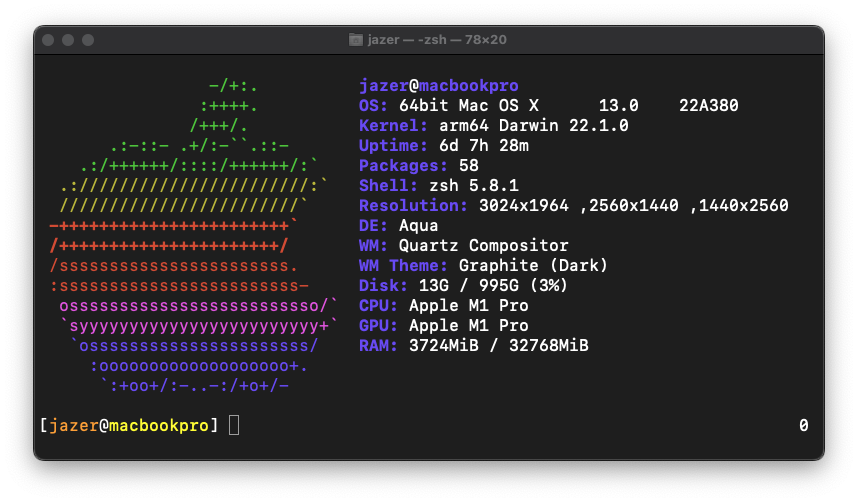
\includegraphics[width=\linewidth]{macos-screenshot.png}}
    \caption{Screenshot of MacOS computer statistics used in development}
    \label{fig:macos}
\end{figure}

MacOS (Figure~\ref{fig:macos}) was the primary choice with its native UNIX command line support for operations \parencite{robbins_unix_2006} and ease of use. This capability helped when running build, test and deployment scripts. Windows also provide this through the Windows Subsystem for Linux \parencite{ionescu_alternatives_2019}; however, it is more complex to set up and interface with Windows applications increasing development time.

In addition to this, MacOS natively supports the Safari browser, which is one of the primary browsers in public use. This support is essential during testing alongside other popular browsers available.


\subsection{Editor - Visual Studio Code}
With the project consisting of three parts, an editor supporting the multiple languages in use and providing methods of operating each is an essential requirement. 

\begin{figure}[ht!]
    \centerline{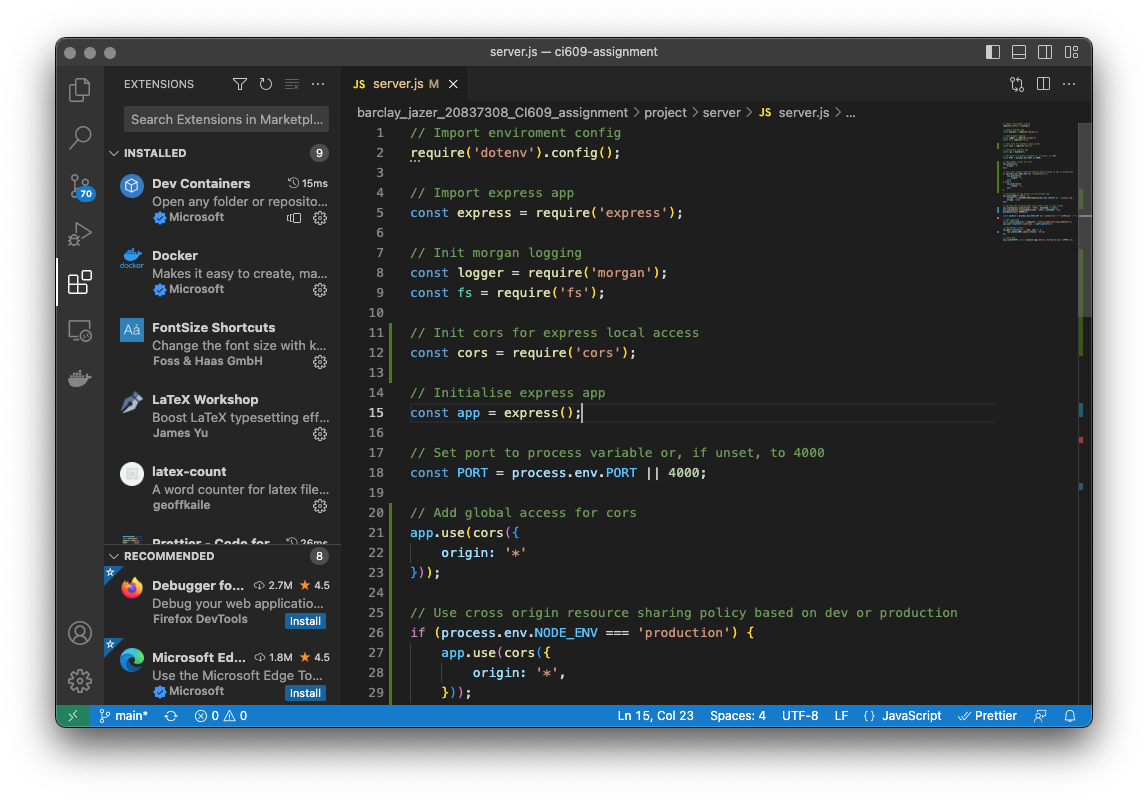
\includegraphics[width=1.1\linewidth]{vscode-screenshot.png}}
    \caption{Screenshot of Visual Studio Code Editor}
    \label{fig:vscode}
\end{figure}

For this reason, Visual Studio Code (Figure~\ref{fig:vscode}) was selected. It is free and provides terminal access from within the development environment to run each part of the project. It also has extensions for syntax highlighting and IntelliSense for each language, reducing development time looking for language specifications or documentation.

Other editors were considered, such as Notepad++, Atom and Sublime. None of these editors had the same features or support VS Code provided at zero cost.


\subsection{Version Control -- Git and GitHub}
A version control system \parencite{zolkifli_version_2018} provides a historical view of changes made to a project's code and a backup of these changes when stored remotely. It enables developers to make experimental changes on new branches without affecting the functional code in a core branch.

\begin{figure}[ht!]
    \centerline{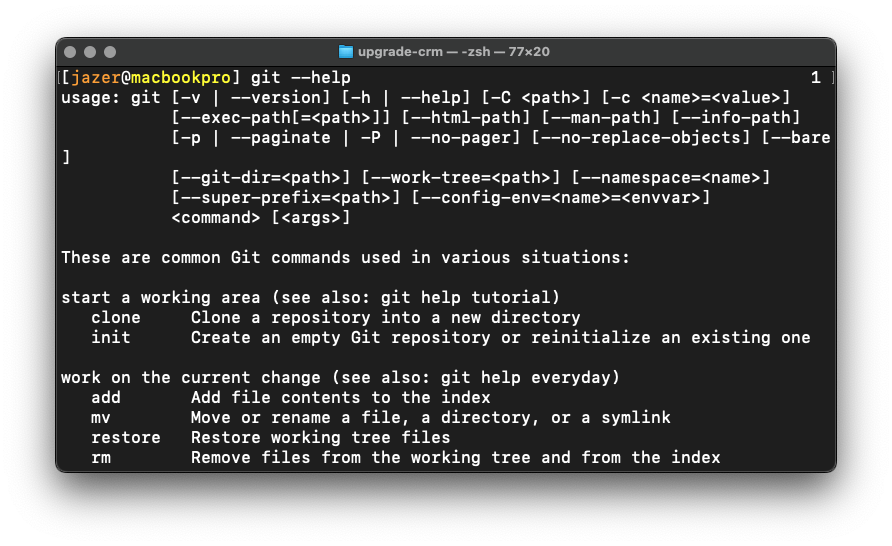
\includegraphics[width=.8\linewidth]{git.png}}
    \caption{Screenshot of Git Help Output}
    \label{fig:git}
\end{figure}

Git \parencite{chacon_pro_2014} was selected for its local and remote storage capabilities (Figure~\ref{fig:git}). It came pre-installed with the operating system as a command line tool. It had a vital role in creating local test branches, which were rebased and merged into the main committed branch.

\begin{figure}[ht!]
    \centerline{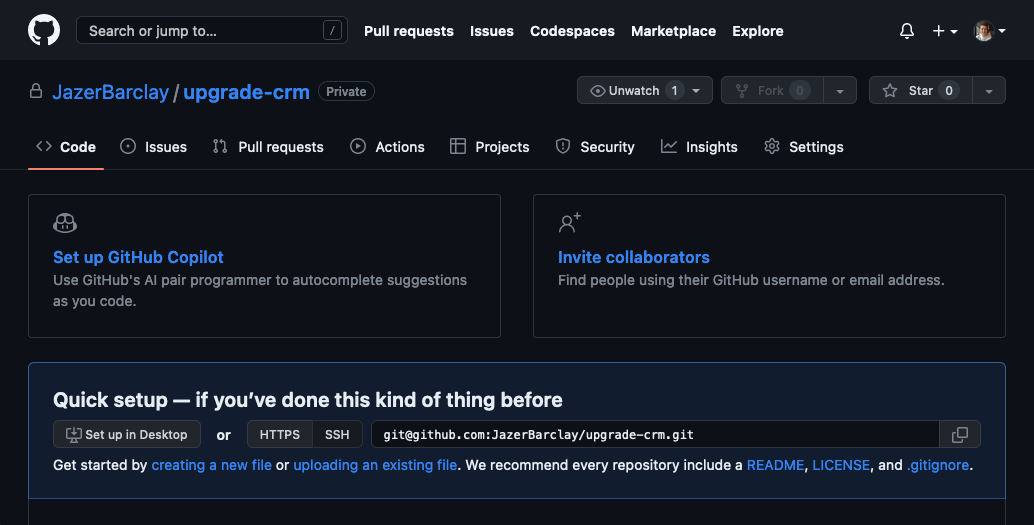
\includegraphics[width=\linewidth]{github.png}}
    \caption{Screenshot of GitHub repository when intialised}
    \label{fig:github}
\end{figure}

GitHub was used with Git \parencite{tsitoara_beginning_2020} to upload the project to the internet (Figure~\ref{fig:github}). This allowed the download of the project to other devices for testing and provided resiliency in the event of a system failure. GitHub also added value through workflows which automated testing when code was uploaded.

Other version control systems, such as SVN \parencite{pilato_version_2008}, were considered for this project but needed more essential features, which Git already provided. In the case of SVN, there is no local history storage, thus requiring an internet connection and online server to track changes. In addition, all history would be lost if the online copy were corrupted or lost.

Other free online Git hosting services exist, such as GitLab, which provides self-hosting options but does not have the same ease of use that Github provides.


\subsection{Web Browser -- Firefox}
Web-based projects require a browser for viewing and testing. Although many were used in the project's testing phase, one was selected for use during development.

\begin{figure}[ht!]
    \centerline{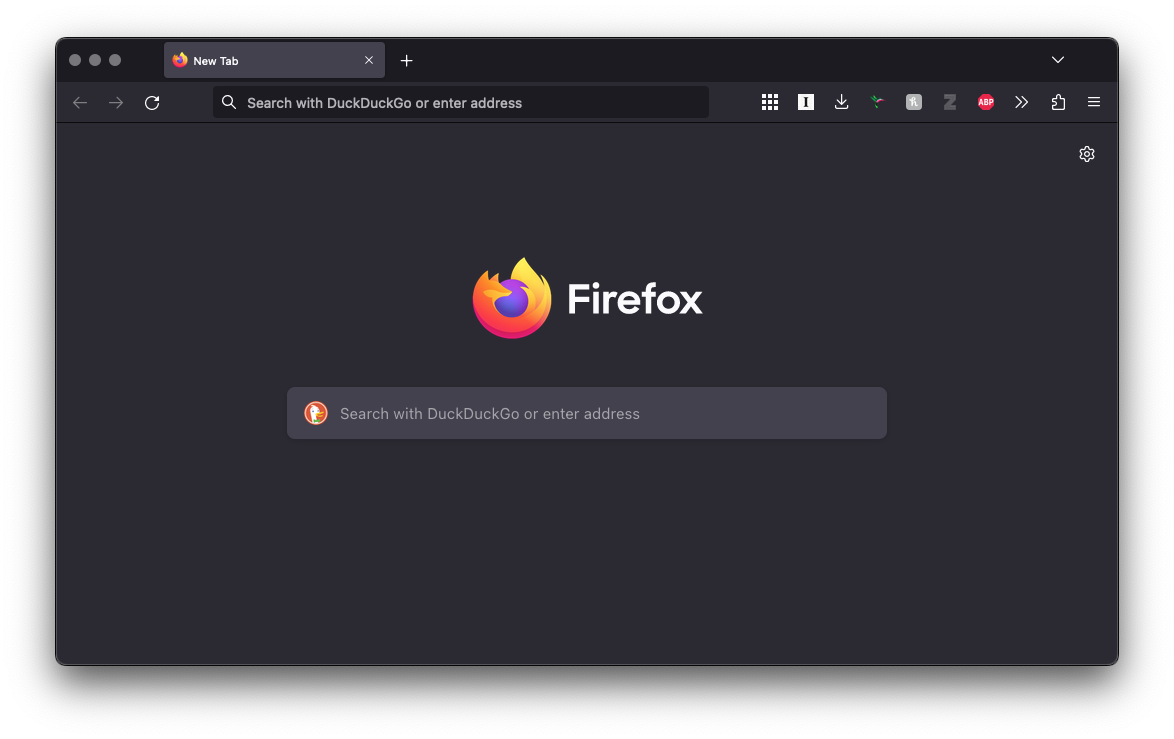
\includegraphics[width=1.1\linewidth]{firefox.png}}
    \caption{Screenshot of the Firefox Web Browser}
    \label{fig:firefox}
\end{figure}

Firefox (Figure~\ref{fig:firefox}) was primarily used with its feature-rich developer support providing a built-in console, page layout viewer and view of local storage variables. Other browsers were later used for testing to ensure the system functions across all, including Google Chrome, Safari, Opera and Microsoft Edge.


\subsection{API Interaction -- Postman}
An API was used to interface with the database. The web browser can interact with the API, albeit crudely and with limited functionality.

\begin{figure}[ht!]
    \centerline{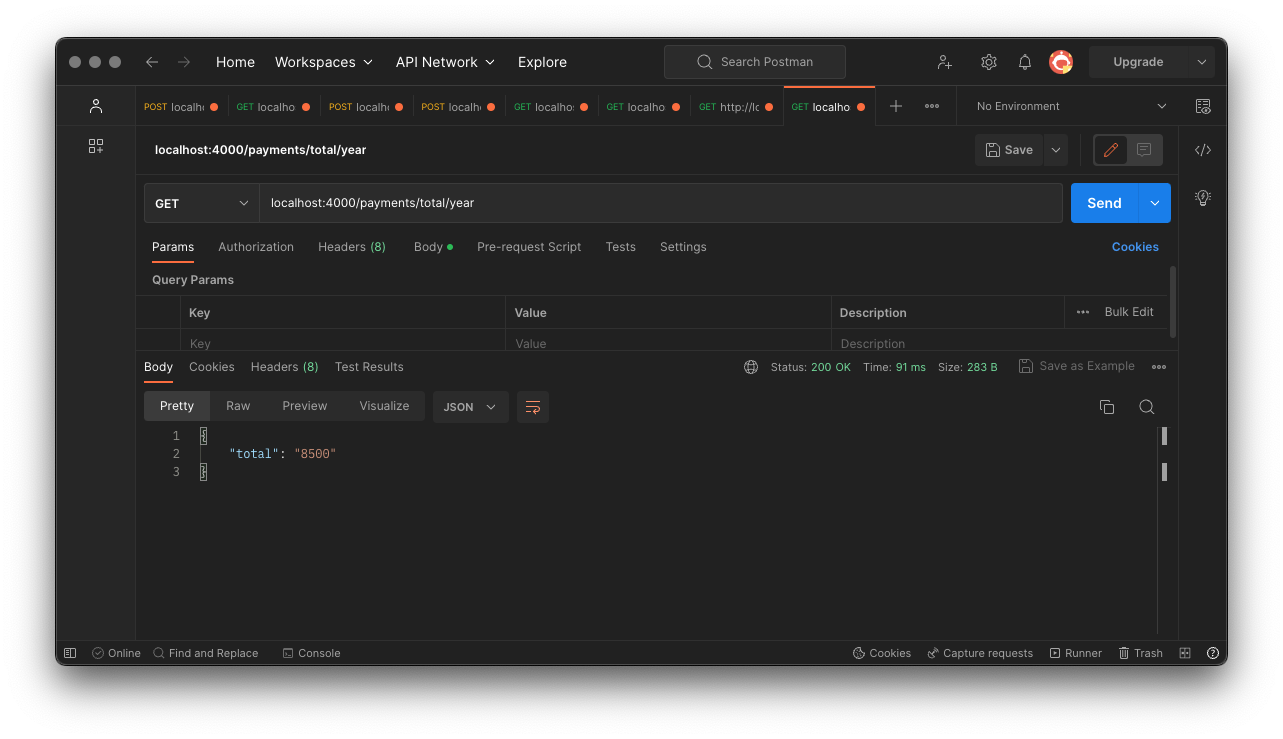
\includegraphics[width=.9\linewidth]{postman.png}}
    \caption{Screenshot of the Postman API Tool}
    \label{fig:postman}
\end{figure}

Postman (Figure~\ref{fig:postman}) was utilised for crafting custom API requests and automated black box testing requests for edge and error cases to aid in the development and testing of the API.


\subsection{Database Management System -- PostgreSQL}
A database management system allows direct access and manipulation of data stored in a database without requiring a recompilation. This access is valuable during development for quick modifications, testing data storage types and links between tables.

\begin{figure}[ht!]
    \centerline{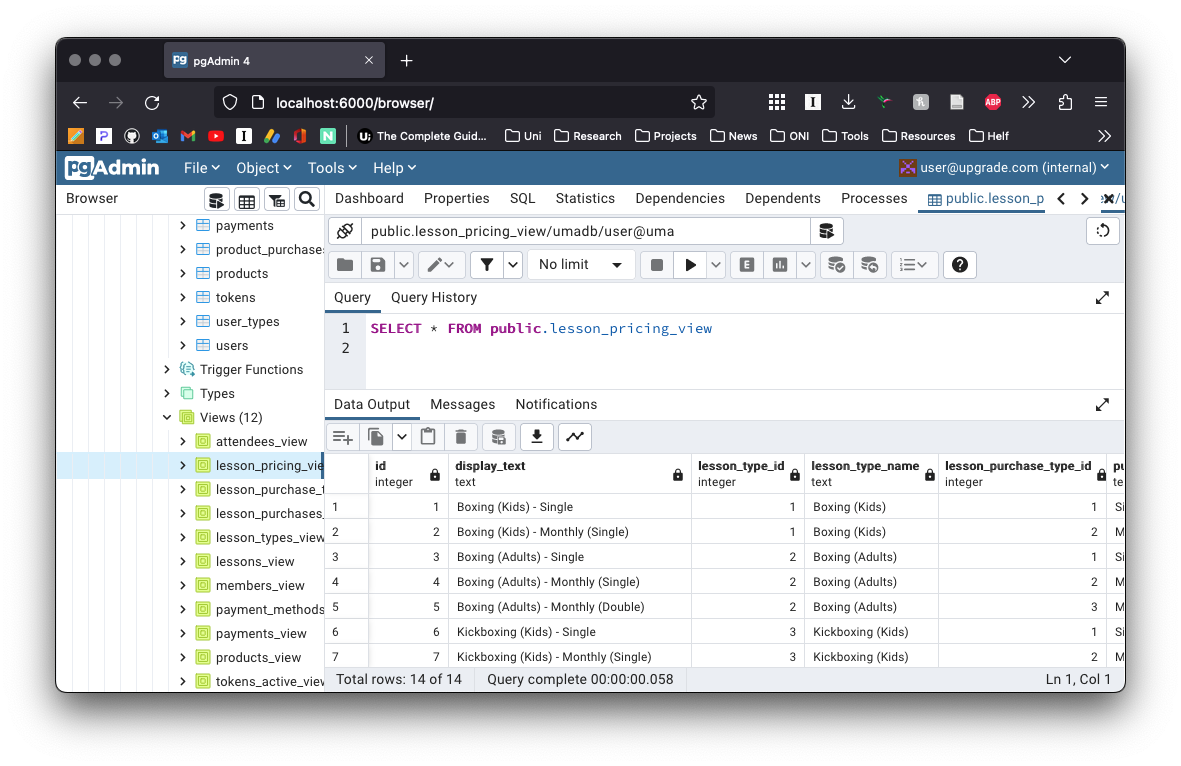
\includegraphics[width=.9\linewidth]{pgadmin.png}}
    \caption{Screenshot of PgAdmin4 Interface for Accessing the Database}
    \label{fig:pgadmin}
\end{figure}

With PostgreSQL within Docker providing the database for this project, the PgAdmin4 tool (Figure~\ref{fig:pgadmin}) was utilised within the same Docker environment. PgAdmin includes analytics to the PostgreSQL database and table creation and modification tools.

Other tools exist to interface with a database however are very generic and designed to operate with any relational database.


\subsection{Deployment - Docker}
Docker (Figure~\ref{fig:docker}) standardised testing and deployment environments to contain each project segment through the use of containers \parencite{merkel_docker_2014}. Each component could be tested individually for errors and rebuilt for deployment on the development or live server when changes were made.

\begin{figure}[ht!]
    \centerline{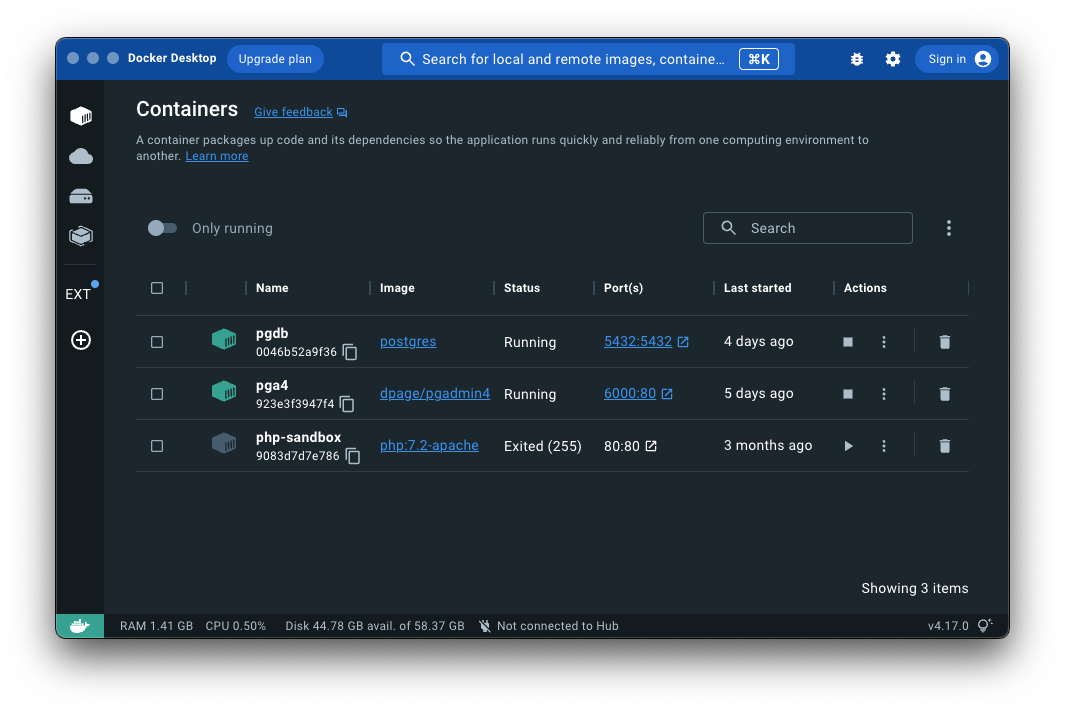
\includegraphics[width=1.1\linewidth]{docker.png}}
    \caption{Screenshot of the Docker Dashboard with Running Containers}
    \label{fig:docker}
\end{figure}

\subsection{Project Tracking -- Trello}
Maintaining progress through the project lifecycle is vital to remain on track and within the time constraints. The software must be flexible to fit the developer's approach while remaining uncomplicated.

\begin{figure}[ht!]
    \centerline{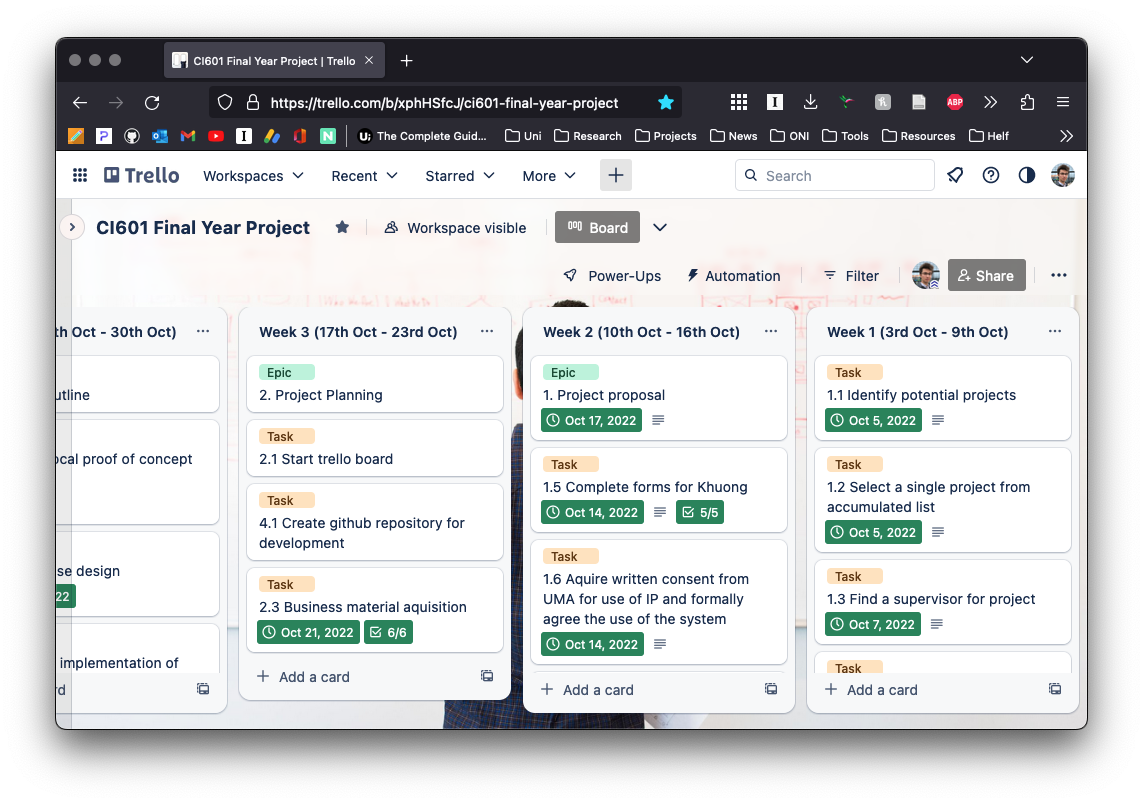
\includegraphics[width=1.1\linewidth]{trello.png}}
    \caption{Screenshot of Trello Running in Firefox}
    \label{fig:trello}
\end{figure}

Trello (Figure~\ref{fig:trello}) was selected to track the project's progress from inception to creation. It is an online Kanban board system designed to support lists and cards. Having a visual display of the features to be added, the current work in progress, and what has been completed each week provides great insight helping with time estimates with work and keeping work only to the tasks which move the project closer to its goals.

Atlassian also provided a tool designed specifically for agile and the scrum approach. However, it was more complicated and geared towards collaboration rather than simple project management.


%----------------------------------------------------------------------------------------
%	2. Development approach
%----------------------------------------------------------------------------------------

\section{Development approach}
There are many approaches developers and businesses may use to structure software development, each with its benefits and drawbacks. With this project being a solo endeavour, a system primarily focused on collaboration would be less beneficial than one designed to deliver features.

Since this project has a short timeframe and an end date, non-iterative approaches such as the waterfall method (Figure~\ref{fig:water}) would be unproductive \parencite{mpcs_waterfall_2012}. Feedback from the business owners and supervisor, including bug fixes and edge cases, would not be actionable and require a new development stint beyond the project's deadline.

\begin{figure}[ht!]
    \centerline{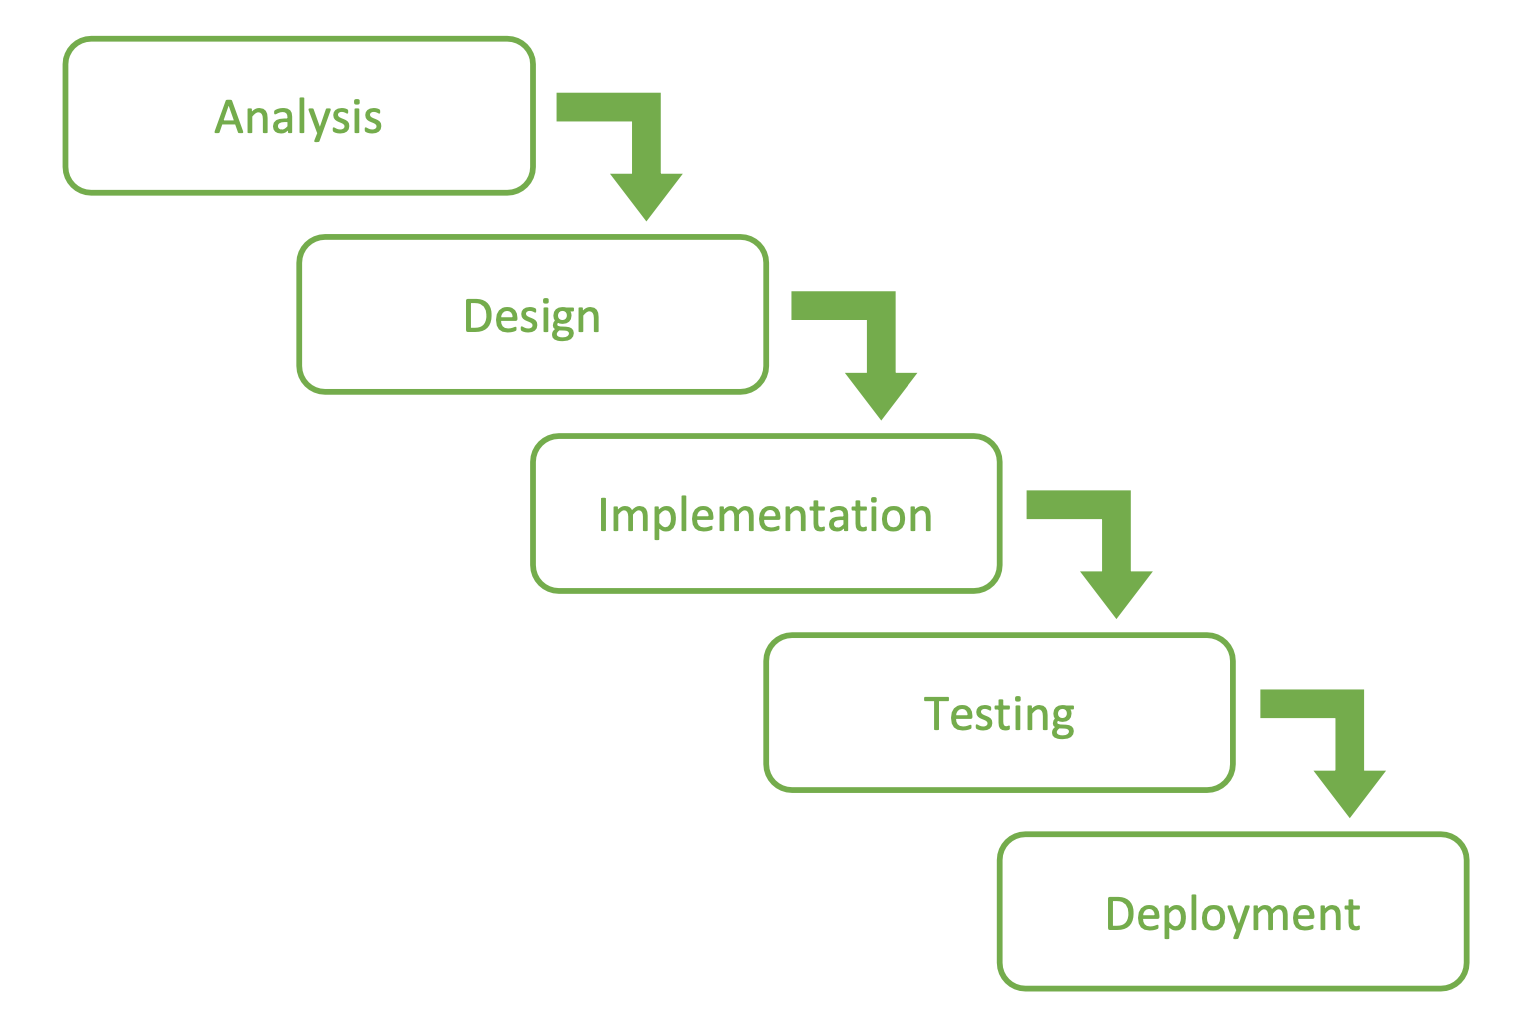
\includegraphics[width=.9\linewidth]{waterfall.png}}
    \caption{The Waterfall Development Method}
    \label{fig:water}
\end{figure}

Agile \parencite{shore_art_2022} (Figure~\ref{fig:agile}) and Feature Driven Development (FDD) (Figure~\ref{fig:fdd}) were the two promising strategies for this project. The agile approach is designed more for teams however emphasises regular meetings with stakeholders and project managers. FDD, on the other hand, is about delivering features in a more structured manner with less focus on a team \parencite{lucid_why_2019}.


\begin{figure}[h!]
    \centerline{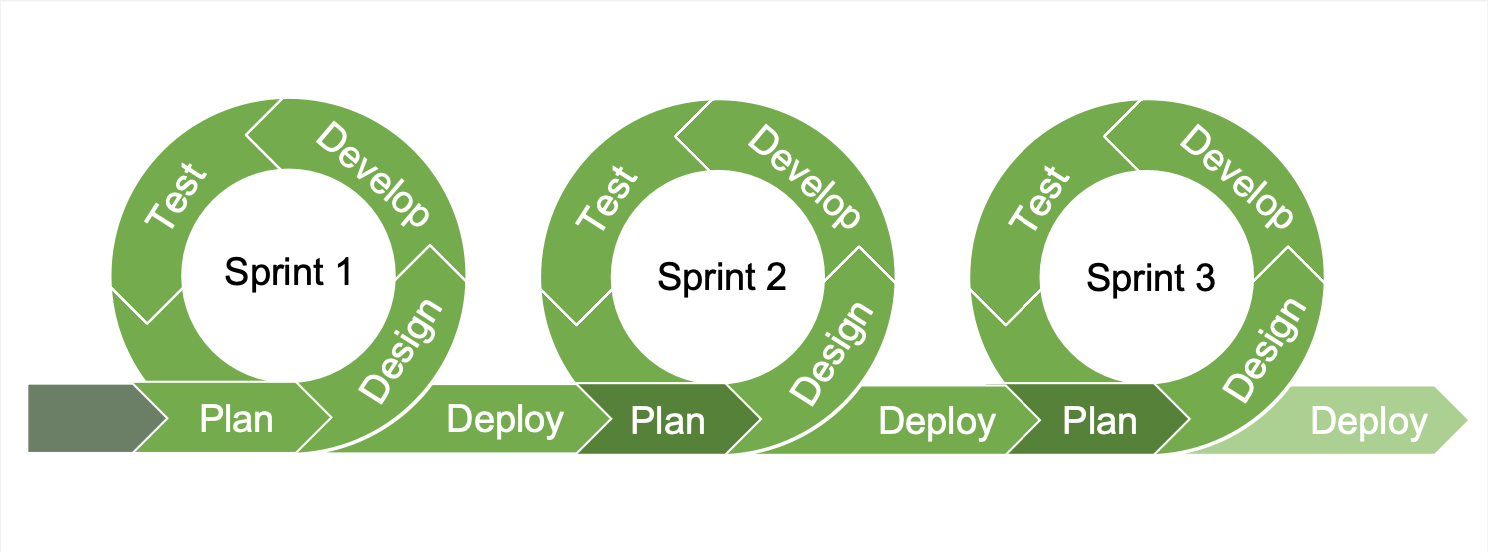
\includegraphics[width=1.1\linewidth]{agile.png}}
    \caption{The Agile Iterative Development Method}
    \label{fig:agile}
\end{figure}

\begin{figure}[h!]
    \centerline{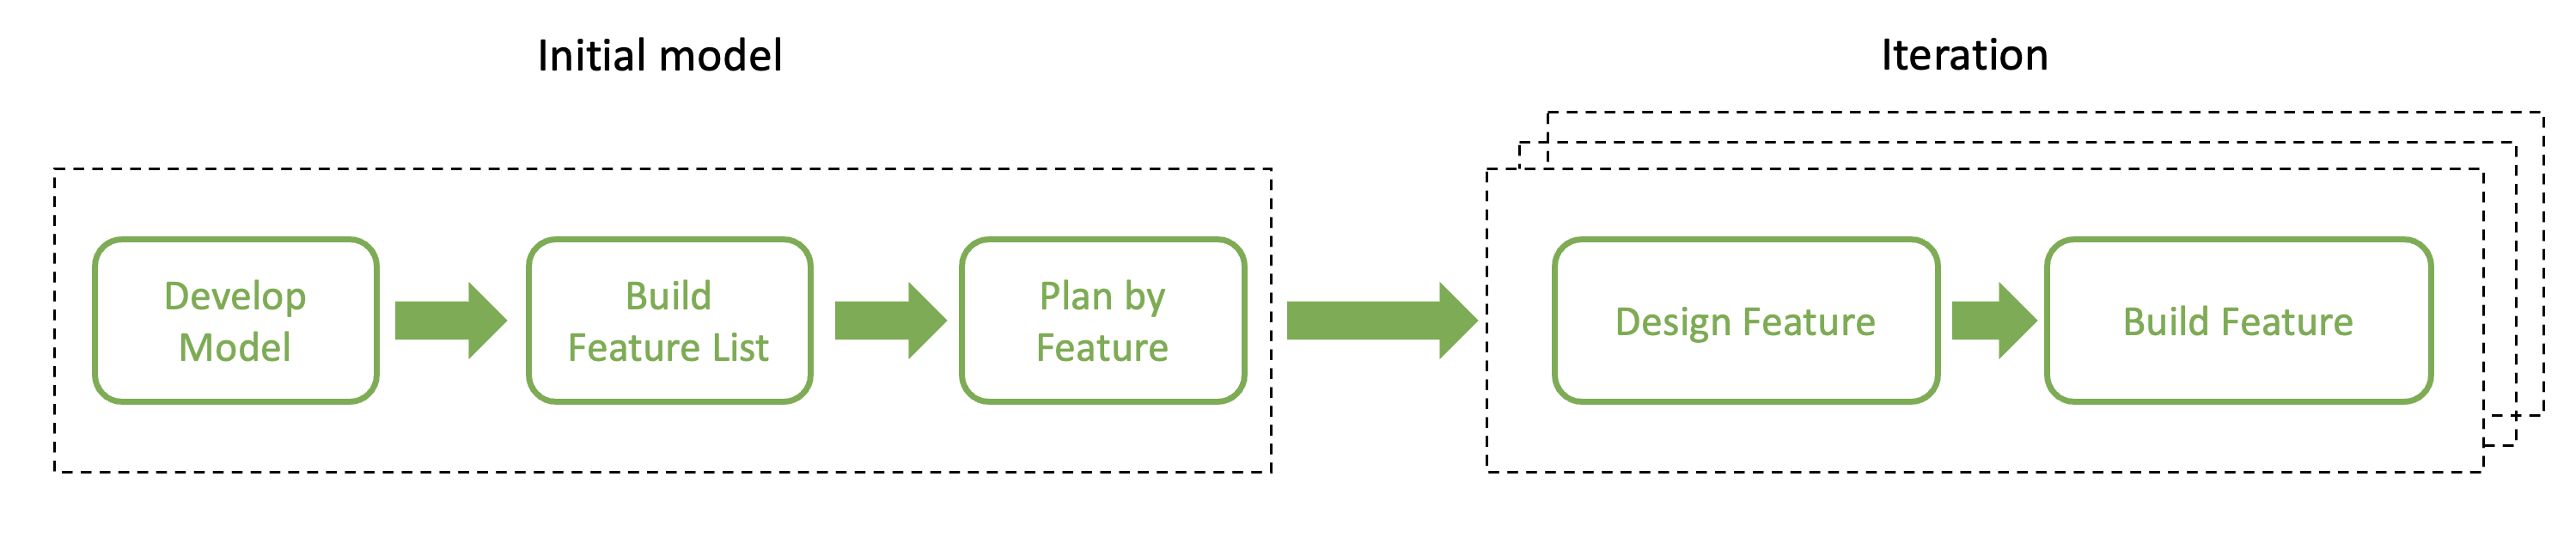
\includegraphics[width=1.1\linewidth]{fdd.png}}
    \caption{The Feature-Driven Development Method}
    \label{fig:fdd}
\end{figure}

Both provided certain qualities that the project development structure would require. However, no specific structure or approach is set in stone; As a result, a mixture of both was employed \parencite{sremath_tirumala_hybrid_2016}. Agile qualities, including sprints, regular check-ins with the supervisor and business managers, and a feature delivery focus structure from FDD, were ultimately used when building the software.

This structure can be seen in the Gantt charts (Figures~\ref{fig:gantt1} and~\ref{fig:gantt2}) created at the beginning of the project, splitting work into an initial development stage before the winter break and bi-weekly sprints where new features are added for greater functionality.

\begin{figure}[ht!]
    \centerline{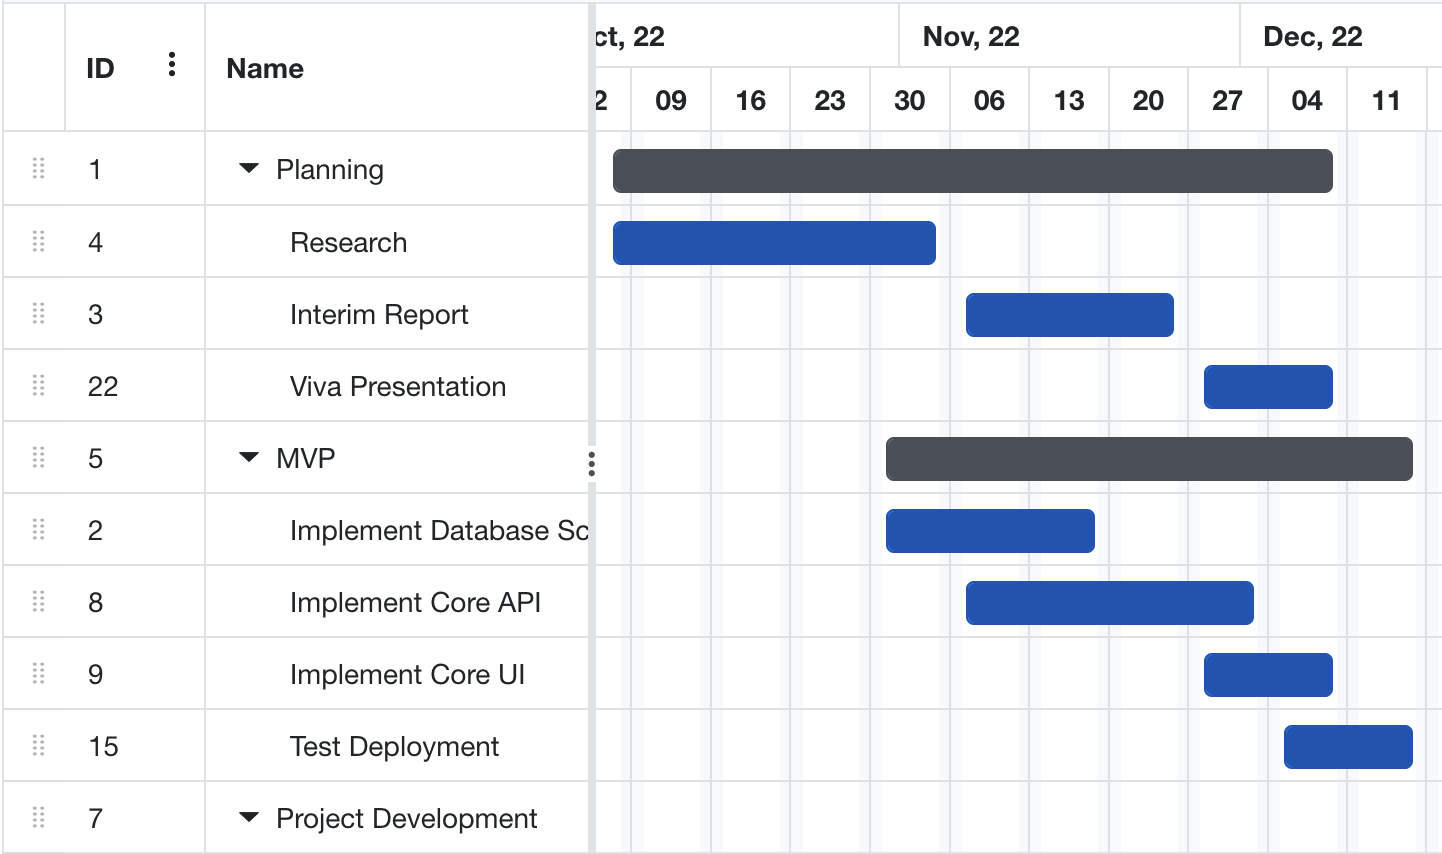
\includegraphics[width=1\linewidth]{gantt1.png}}
    \caption{A Gantt Chart of the planning phase of this Project}
    \label{fig:gantt1}
\end{figure}

\begin{figure}[ht!]
    \centerline{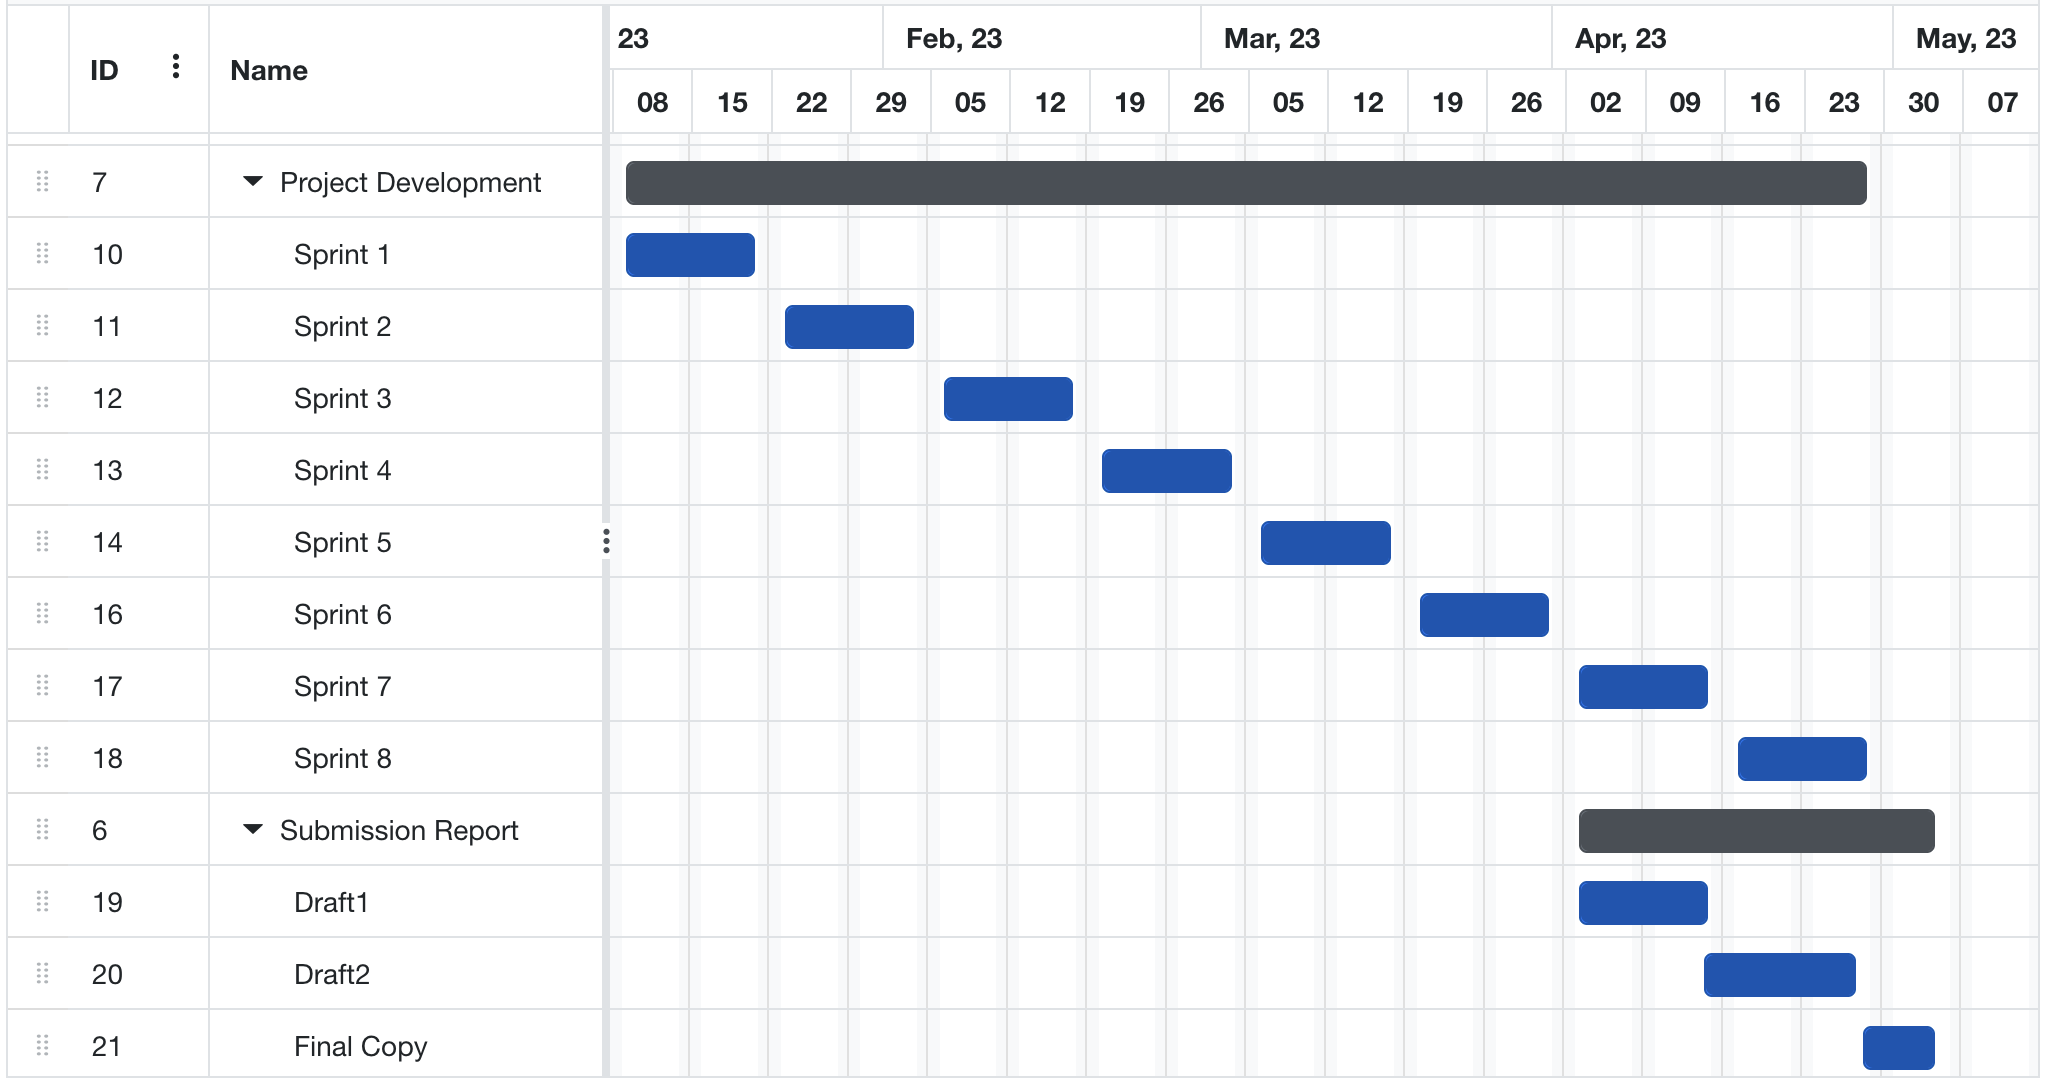
\includegraphics[width=1\linewidth]{gantt2.png}}
    \caption{A Gantt Chart of the sprint development phase of this Project}
    \label{fig:gantt2}
\end{figure}

A further breakdown of the work completed in the initial stages and the bi-weekly sprints is available through the tracked progress in Trello.

\begin{figure}[ht!]
    \centerline{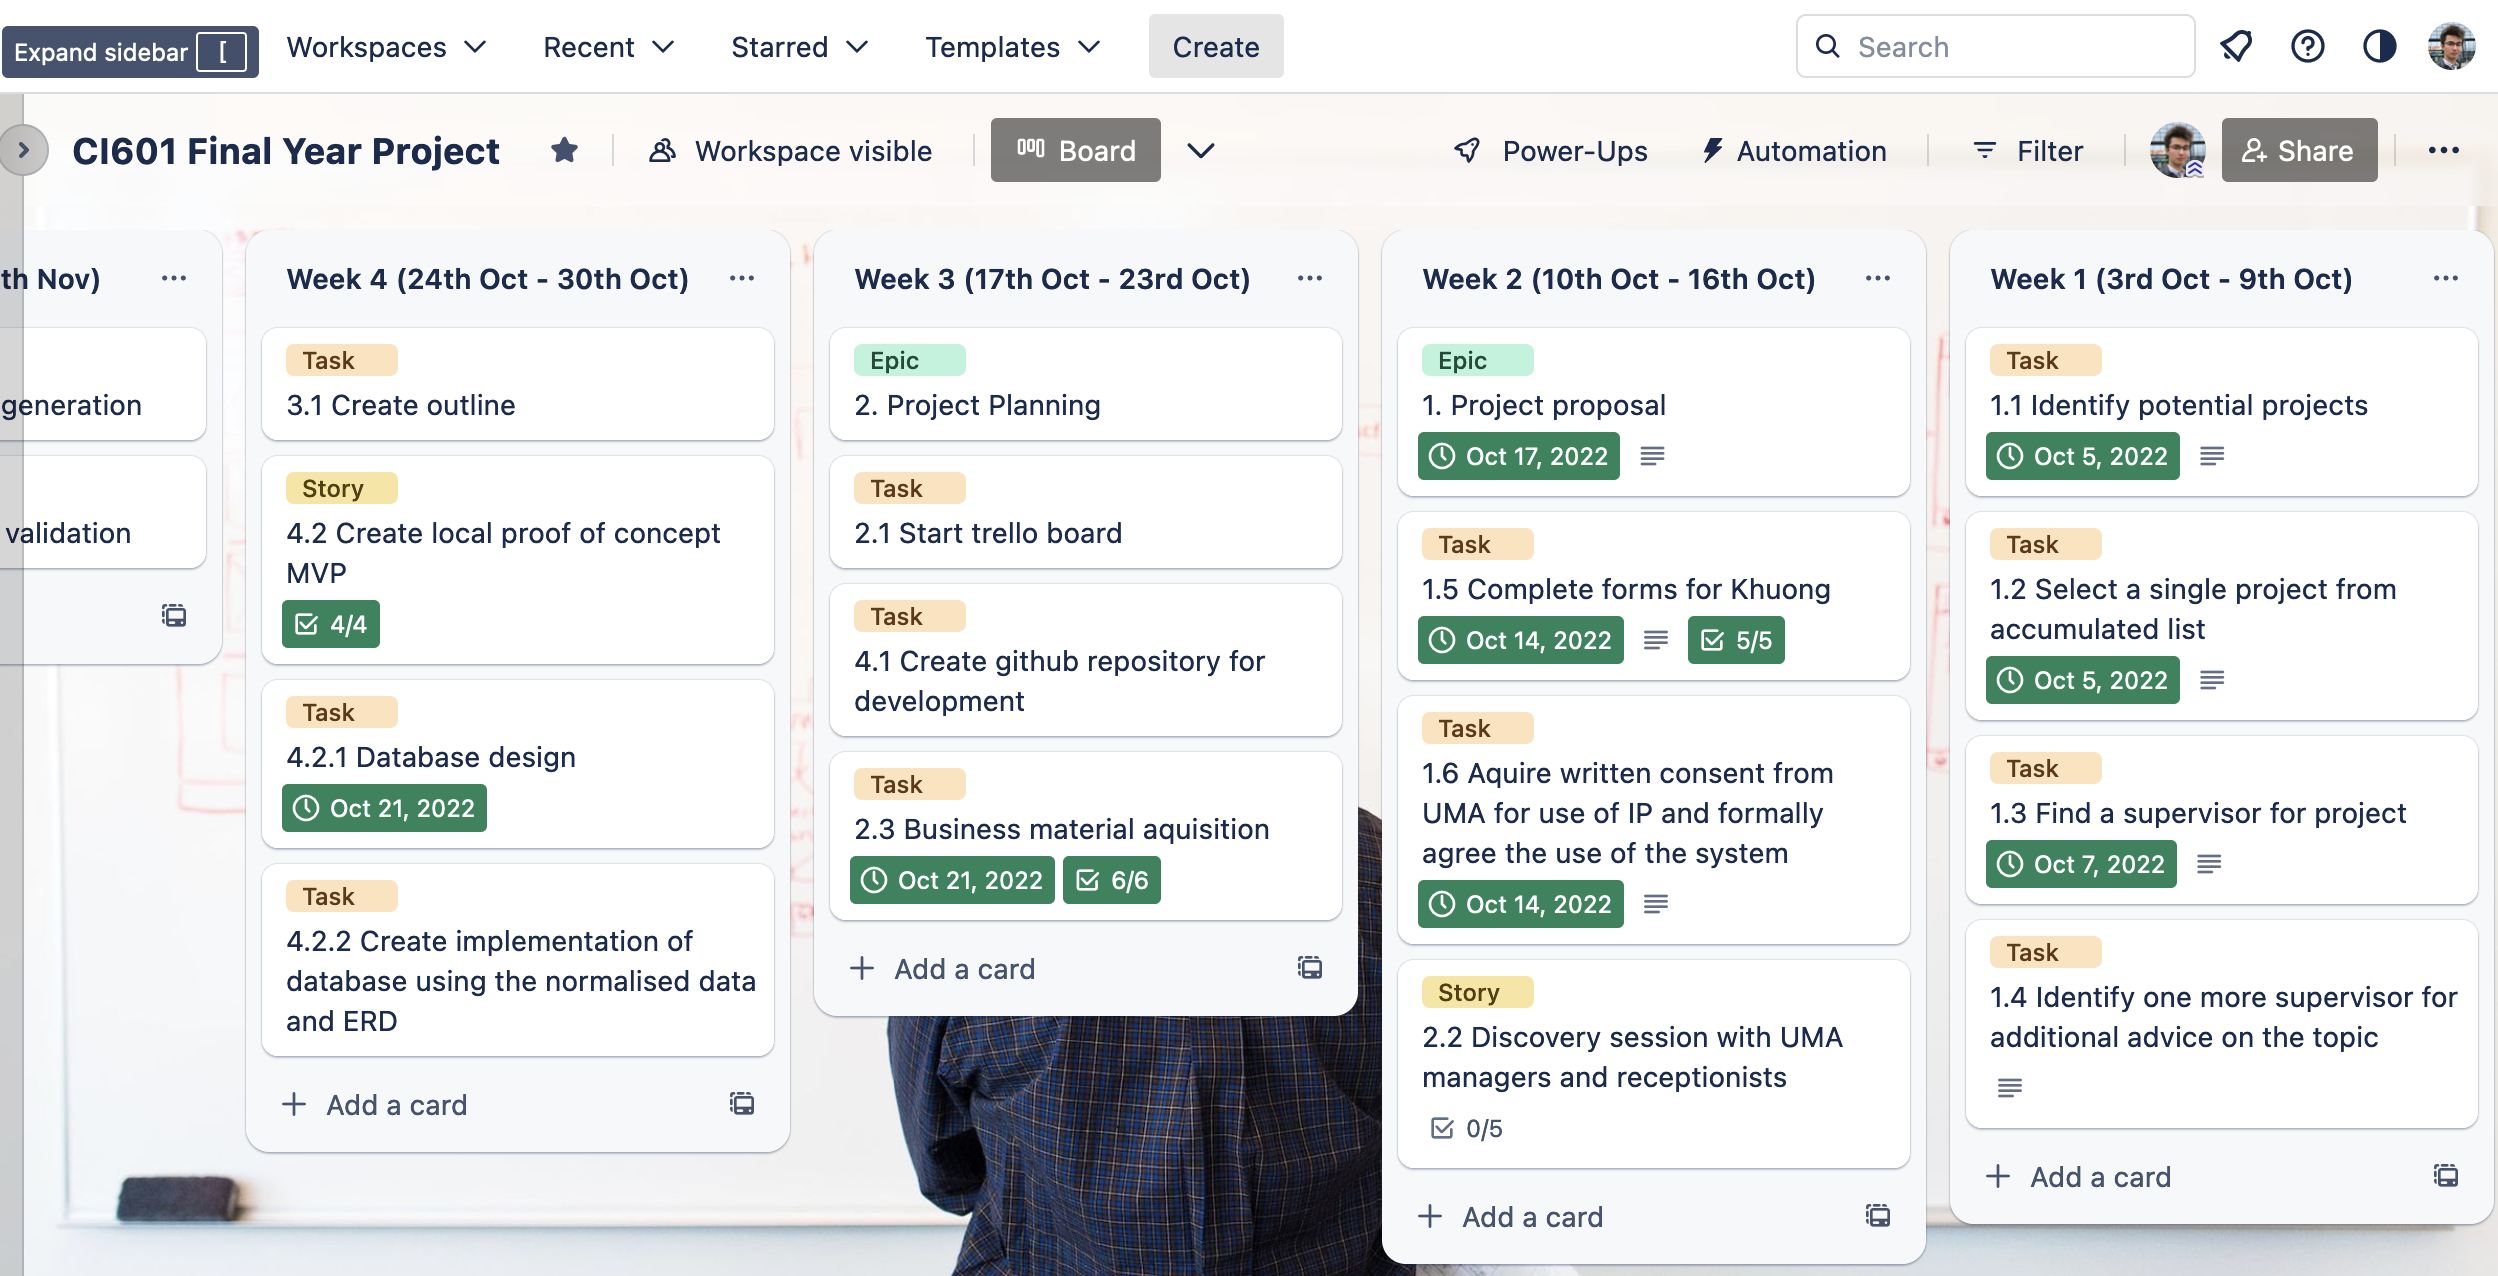
\includegraphics[width=1\linewidth]{trello-first.png}}
    \caption{Screenshot of First 4 Weeks Tracked on Trello}
    \label{fig:trello-board}
\end{figure}